\Chapter{Koncepció}

\Section{Kiterjesztett valóság}

% TODO: A dolgozat témája hogyan kapcsolódik hozzá, és hogy általában mit értünk alatta.

A kiterjesztett valóság (\textit{Augmented Reality}, AR), mint fogalom alatt olyan érezékelhető valóságot értünk, amelyben a valós és virtuális elemek keverednek és a virtuális elemekre a valódi világ hatással van. A virtuális valóssággal (\textit{Virtual Reality}, VR) ellentétben, ahol az érzékelt valóság teljes mértékben digitális, az AR-nek a környezetét a valós világ adja, azzal szoros kapcsolatban áll és, mint a nevében is benne van, annak egyfajta kiterjesztésével kíván egy új valóságot létrehozni.

Megvalósításának számos módja ismert, gondolhatunk például a legelterjettebb felhasználási területre, az okostelefonos megoldásokra is. A legtöbb közösségi felülethez tartozó kamera-alkalmazások kiterjesztett valóság alapú technológiákat is alkalmaznak, melyek segítségével az előlapi kamera képével a felhasználók az arcukra különböző filtereket, digitális maszkokat illeszthetnek. Megemlíteném még a népszerű játékot is, a \textit{Pokemon Go}-t, melyben a képernyőt nézve nyerhetünk betekintést a kiterjesztett valóságba. Az okostelefon különféle szenzorainak hála (giroszkóp, GPS, iránytű) a kiterjesztett világot bejárhatjuk, a telefon képernyője egy ablakot nyit eme kevert valóságba. Az ilyen megoldásokat \textit{Spatial Augmented Reality}-nek \cite{bimber2005spatial}, vagyis térbeli kiterjesztett valóságnak nevezzük. A virtuális elemek helyzete a valós világ bizonyos pontjaihoz van kötve, a virtuális elemek pedig függenek a valós környezettől.

\begin{figure}[h]
\centering
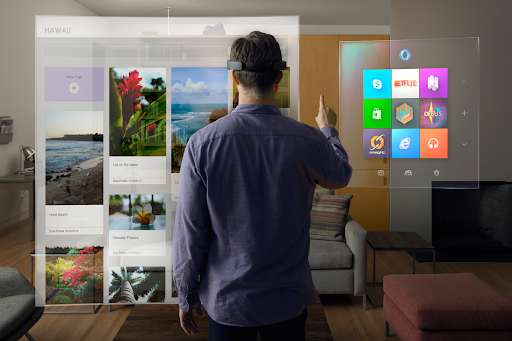
\includegraphics[width=10.3truecm, height=6.28truecm]{images/AR-hololens.png}
\caption{Microsoft HoloLens promóciós kép}
\label{fig:hololens}
\end{figure}

A kevert világ észlelésének módjai történhetnek a már említett kézi eszközökön kívül fejre helyezhető eszközök segítségével is, illetve megvalósulhat külső eszközök használatával is.
A fejre helyezhető eszközök általában olyan speciális szemüvegek, amelyekben a valós és virtuális világ egyformán érzékelhető. Ezen eszközökre is jellemző a már okostelefonoknál említett szenzorok használata a pontosabb eredmény elérése érdekében.

A fejre helyezhető eszközöket két csoportra oszthatjuk:
\begin{itemize}
	\item A valós világot egy kamera képén keresztül érzékeljük és erre a videófolyamra rajzolódnak ki a virtuális elemek. Az ilyen megvalósításokra jellemző az okostelefonok használata is, speciális fejre helezhető keret segítségével. Ez a megoldás rendkívül költséghatékony, hiszen csak a \textit{headset-et} kell beszereznünk. Az ilyen \textit{headset-ek} egyik úttörője volt a Google Cardboard terméke is. Az okostelefonos megoldások egyik hátrányai közé sorolhatjuk a monoszkópikus érzékelését a valós világnak. Viszont a többkamerás készülékek elterjedésével ez a probléma is orvosolható.
	
	\item Egy specális lencsén keresztül érzékeljük a valóságot, melyen megjelennek a digitális tartalmak. Ilyen eszköz például a \textit{Microsoft HoloLens} is.
\end{itemize}

A külső eszközökkel megvalósított kiterjesztett valóság, amelyet több személy is eszközök nélkül is egyaránt megfigyelhet, a különböző projektorok, hologrammok és egyéb speciális technikák alkalmazásával valósulhat meg.

Egy másik megközelítés lehet a már okostelefonoknál említett megoldás felnagyított valtozata is, fix kamerával és nagyobb képernyővel. Ha pedig a kamera képét függőlegesen tükrözzük, akkor olyan hatást érhetünk el, mintha egy tükrön keresztül vizsgálnánk a körülöttünk létrehozott kevert valóságot. A tükör képe a videófolyam, amelyet virtuális elemekkel egészítünk ki, a telefonos megoldáshoz hasonlóan.
A dolgozatomhoz elkészített programom vezérlése szempontjából ezen megoldása tűnt a legmegfelelőbbnek. A prezentáló személy a tükörképe segítségével kapcsolatba tud lépni a kiterjesztett valósággal és annak elemeivel, így irányítva a program működését.

\Section{Prezentációs szoftverek}

% TODO: Megnézni 3-6 hasonló szoftvert. Készülhet hozzá összehasonlító táblázat, képernyőképek.

Manapság számtalan prezentációs szoftver közül választhatunk. A legtöbb szoftverről elmondható, hogy diasoros elven működik, vagyis a prezentáció anyaga egy előre meghatározott sorrendben fut le, a tartalom elemek pedig ún. fóliákon helyezkednek el, hasonló módon, mint a régi írásvetítők esetében, ahol a prezentáció témáját előre elkészített fóliák segítségével mutathattuk be. Manapság már a prezentáció anyaga teljes mértékben digitális, viszont a hagyományos értelemben vett prezentációs szoftverek esetében a vetítés menete hasonló, a digitális fóliákat cserélgethetjük, lépkedhetünk közöttük.

A digitális tartalom lehetőséget ad arra, hogy dinamikus elemekkel ellátott, látványos prezentációt készítsünk. Erre a különböző szoftverek különféle lehetőségeket kínálnak.
Az egyik legismertebb prezentációs szoftver kétségkívül a \textit{Microsoft PowerPoint}. Meghatározó szereplője a prezentációs szoftverek világának. Használatával gyorsan és egyszerűen állíthatunk össze prezentációkat, amelyek minőségét a látványos átvezető animációk és a dinamikus elemek használatával fokozhatunk. Hátrányai közé tartozik a platformfüggőség és a magas ára is.

\begin{figure}[h]
\centering
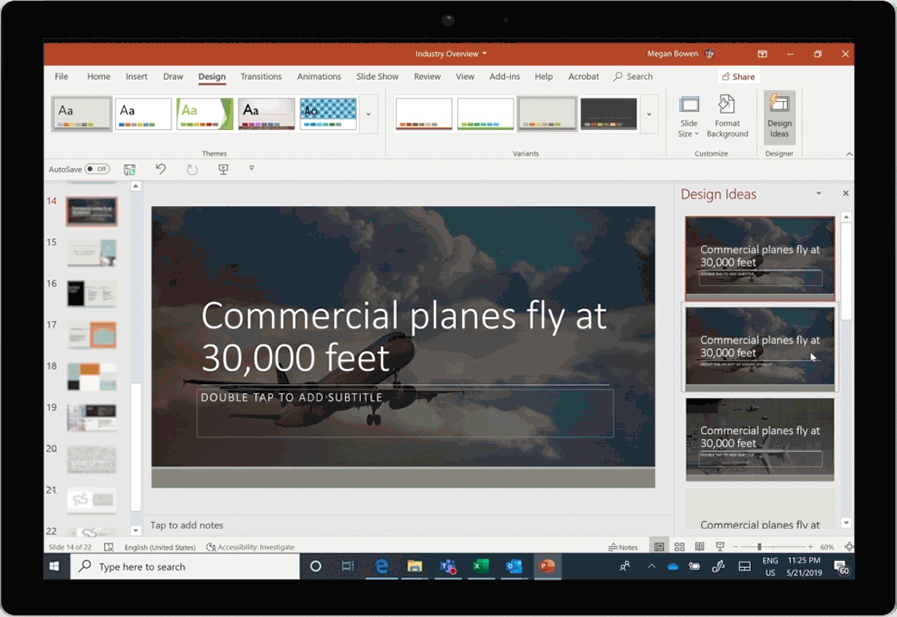
\includegraphics[width=8.97truecm, height=6.17truecm]{images/PowerPoint.png}
\caption{Képernyőfotó a PowerPoint-ről (forrás: microsoft.com)}
\label{fig:ppt}
\end{figure}

Több, hasoló elven működő ingyenes szoftver is megjelent az évek során, amelyek képesek kezelni a PPT formátumát is. Ezen szoftverek segítségével megoldhatjuk a kompatibilitási gondokat. Mivel ingyenesek és platformfüggetlenek, mindenki számára elérhetőek. Megemlíthetném a sok közül a \textit{Libre-Office}-t, a \textit{WPS-Office}-t és a \textit{Google Slides}-ot. Működésük nagyban hasonlít a \textit{Power Point}-hoz, utóbbit internetkapcsolat mellett a böngénszőnkben használhatjuk.

A diasoros prezentációs szoftverek világán túl is léteznek izgalmas megoldások. 
Ilyen a \textit{Prezi} szoftvere is, mely újítása egy egyszű koncepció nagyszerű megvalósítása: A tartalmat egy nagymértű virtuális vászonra helyezhetjük el, majd megadhatjuk, hogy a nézőpont mely pontok között ugráljon. Így olyan hatást érhetük el, mintha a lebegnénk a virtuális vászon fölött. Ha szeretnénk lehetőségünk van megmutatni a teljes vásznat is. A \textit{Prezi} a korábbi megoldások lineáris kötöttségét kívánta eltörölni. Használatával egyedi és látványos bemutatókat készíthetünk. Az ingyenes változata internet használata mellett böngészőben használható.
2017-ben a Prezi bejelentette, hogy kiterjetsztett valóságot megvalósító prezentációs szoftvert tervez fejleszteni, \textit{Prezi AR} néven. A beharangozó konferencián kívül az internetre felkerült még pár videó is, amelyekkel a koncepciót kívánták szemléltetni. A tervek szerint a prezentáló a videófolyamra rajzolt virtuális elemek segítségével mutathatja be a témakört. A közzétett demo videók alapján kapcsolatba is léphet ezekkel az elemekkel a gesztusai segítségével. A projektről azóta semmiféle hír nem jelent meg.

A kiterjesztett valóság adta lehetőségek alkalmazása prezentációs szoftvereknél egy friss kutatási terület. A \textit{Interactive Body-Driven Graphics for Augmented Video Performance} címen, 2019-ben megjelent publikáció egy megközelítését kívánja bemutatni. \cite{saquib2019interactive}

\begin{figure}[h]
\centering
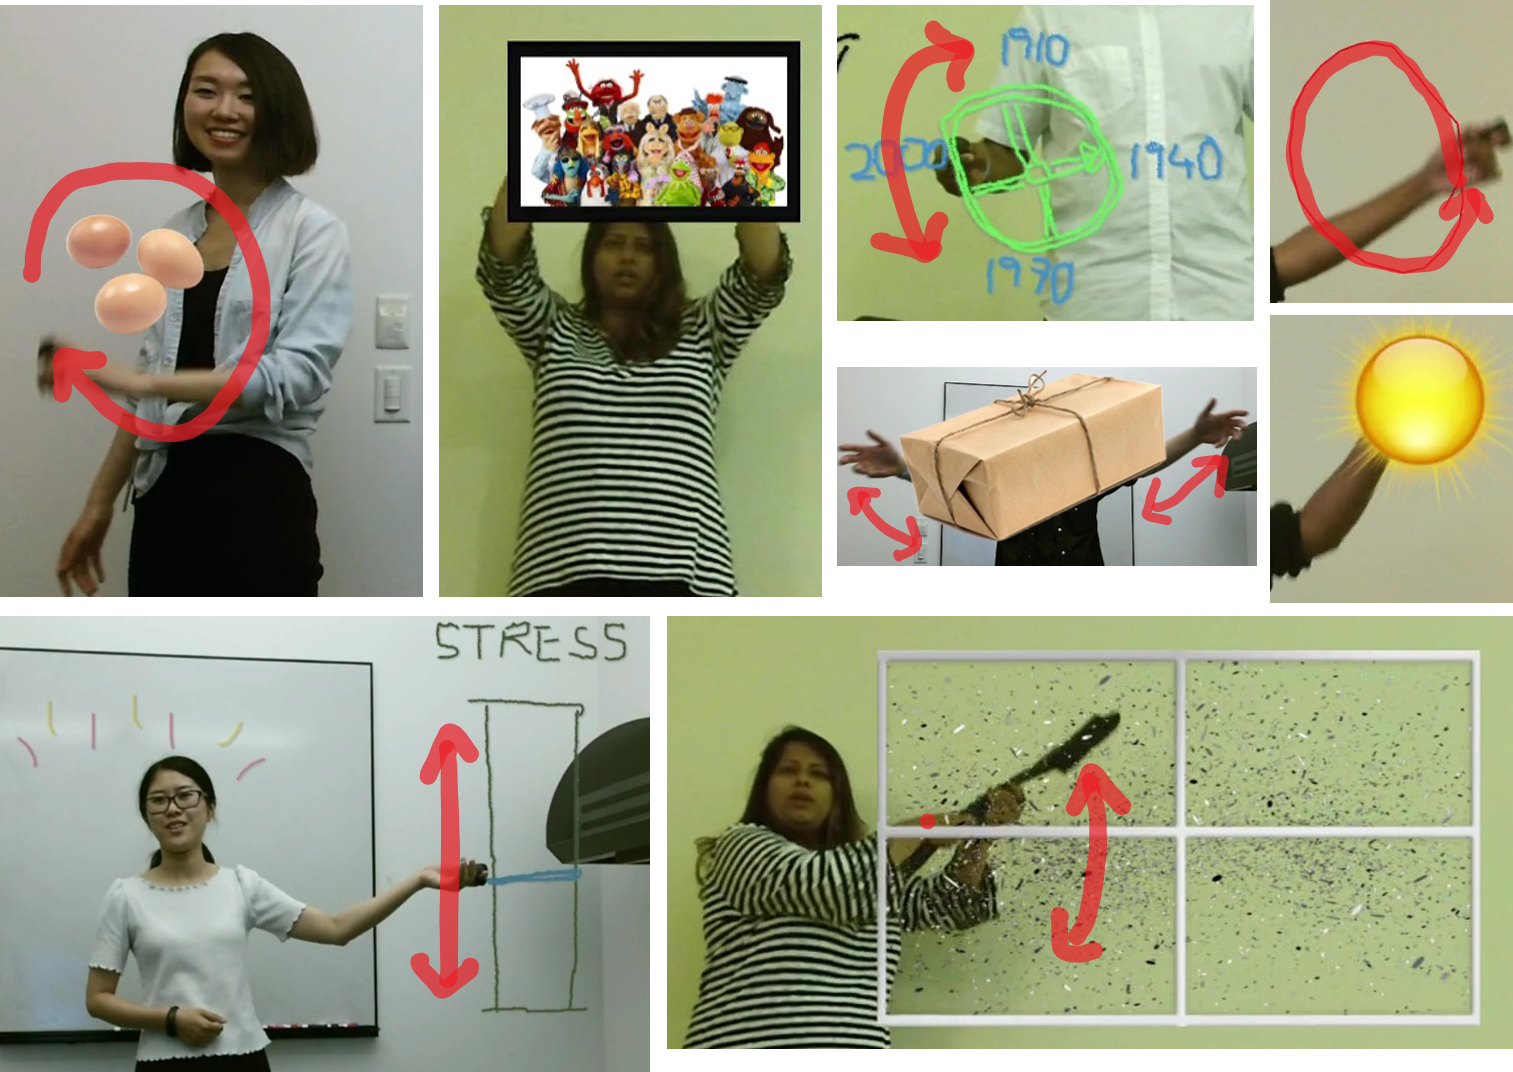
\includegraphics[width=10truecm, height=7.14truecm]{images/IBDGAVP.png}
\caption{Interactive Body-Driven Graphics for Augmented Video Performance}
\label{fig:ibdgavp}
\end{figure}

A megvalósításhoz a \textit{Kinect} kamerarendszert használták fel. Kezdetben \textit{Deep\- -Learning} technológián alapuló alakferismerést kívántak alkalmazni, viszont ez a megoldás még egy magas teljesítményű számítógépen sem tudott kielégítő futási eredményeket adni. A valós idejű futás, amely egy prezentációs szoftvernél elvárt tulajdonság, nem volt lehetséges ezzel a technikával. A szoftver, amelyet használni szerettek volna az \textit{OpenPose} volt, amely magas pontossággal képes megbecsülni a 2D-s videófolyamon elhelyezkedő személyek helyzetét és azok testrészeinek a pozícióját. \cite{cao2018openpose}
A cikkben leírtak szerint a \textit{Kinect} használata megkönnyítette a fejlesztést és segítségével képes valós időben futni a szoftver.

Egy \textit{Widget} szerkesztőt is készítettek a programhoz, amellyel az egérrel vagy digitális rajztáblán rajzolt virtuális elemeket szerkeszthetünk. Az elemekkel a prezentáció során az előadó kapcsolatba tud lépni. A szoftver használata során elengedhetetlen a léptető használata. Ezzel a prezentáló személy egyrészt változtathatja a megjelenített elemeket, aktiválhatja a funkciókat. Másrészt a magyarázó mozgás is jelezhető vele, ilyenkor nem kerülhet interakcióba az elemekkel az előadó.
A publikációban felvetett koncepció hátrányai közé sorolhatjuk az eszközfüggőséget is, vagyis a \textit{Kinect} használatát is (aminek a gyártását 2017-ben felfüggesztették). A \textit{Kinect} mélységérzékelővel ellátott speciális kamerarendszer. Ezen tulajdonsága miatt rendkívül sok kutatáshoz felhasználják. A \textit{Human Computer Interface} és a gesztusfelismerés kutatási területeknél is közkedvelt eszköz. \cite{zhang2013new} \cite{tang2018structured}

% https://simplode.com/home Simplode Suite

\Section{Valós idejű videó annotálás}

Az \textit{OpenCV} egy \textit{open source}, elsősorban valós idejű számítógépes látás megvalósítására támogatást nyújtó, magas tudású függvénykönyvtár. Számos képfeldolgozó algoritmus található benne, melyek implementációjánál a fejlesztők a lehető legjobb teljesítmény elérésére törekedtek.

\begin{figure}[h]
\centering
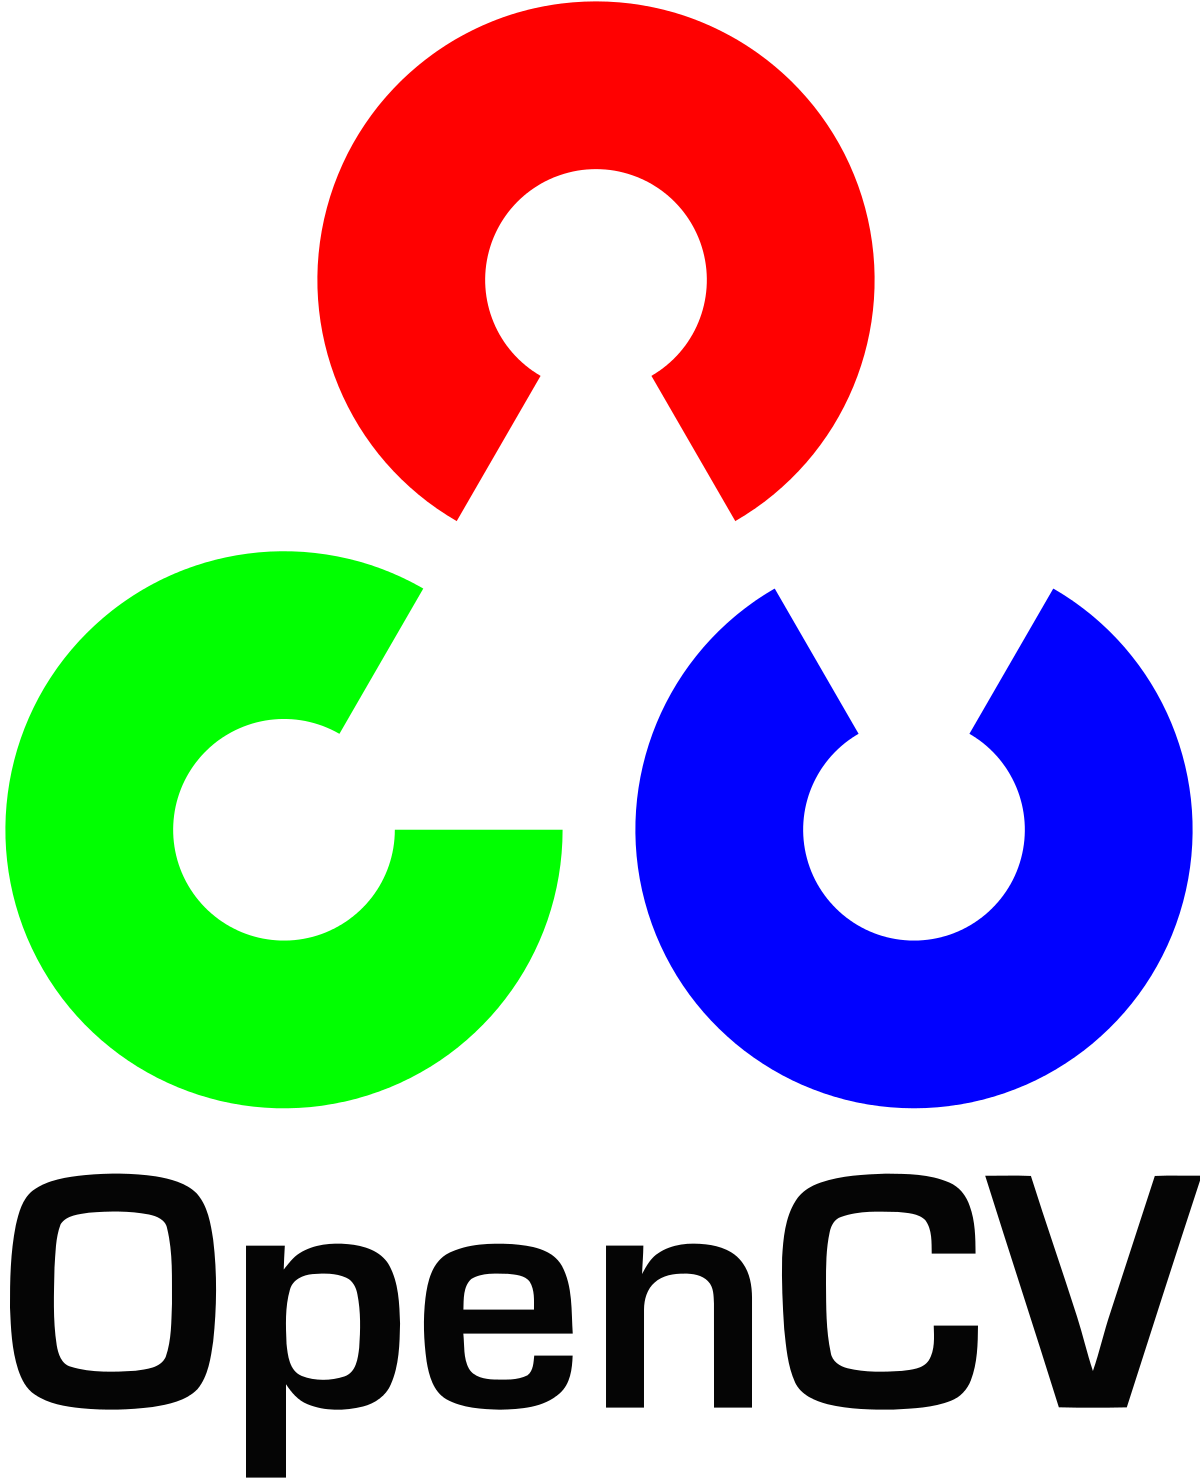
\includegraphics[width=2.4truecm, height=2.96truecm]{images/OpenCV-logo.png}
\caption{Az OpenCV logója}
\label{fig:opencv}
\end{figure}

Az \textit{OpenCV} eredetileg C és C++ nyelven íródott, de különböző nyelveket is támogat, mint például a \textit{Python}-t, \textit{Ruby}-t, \textit{Matlab}-ot, stb\ldots
Platformfüggetlen, így \textit{Linux}-on, \textit{Windows}-on és \textit{Mac OS X} rendszereken is használható. Lehetőséget nyújt továbbá a párhuzamosításra is a \textit{CUDA} és az \textit{OpenCL} technológiák segítségével és tartalmaz egy általános célú gépi tanulásos könyvtárat is, melyek tovább szélesítik a felhasználási területeinek körét. \cite{bradski2008learning}

Videófolyamok feldolgozásához is hasonló eljárásokat alkalmazhatunk, mint az önálló képek esetében. A videó képkockáit iteratív módon dolgozhatjuk fel, képkockáról képkockára. A videó két forrásból származhat: fájból és külső eszközből (pl.: webkamera képe). Az \textit{OpenCV}-ben mindkét esetben először definiálnunk kell egy olvasó eszközt. Ezt \textit{Python} esetében a \texttt{cv2.VideoCapture()} metódussal érhetjük el. Fájlból történő olvasás esetén paraméterként a fájl elérési útvonalára kell hivatkozni, külső eszköz esetén pedig az eszköz \textit{index}-ével történik a hivatkozás. Ha egyetlen ilyen eszköz áll rendelkezésünkre, akkor a 0-ás indexet is használhatjuk, hiszen az az első elérhető eszközre mutató index.
Az eszköz definiálása után a \texttt{.read()} metódusával olvashatjuk ki a képkockákat. A metódus meghívásakor visszatérési értékként megkapjuk a soron következő képkockát és egy értéket, amely az olvasás sikerességéről tájékoztat bennünket. A metódus meghívásakor a videóolvasó pointerét is inkrementáljuk, így a következő \texttt{.read()} meghívásakor már a soron következő képkockát olvashatjuk ki a videófolyamból. Ha már nem kívánjuk tovább használni az adott erőforrást, akkor a \texttt{.release()} metódusával szabadíthatjuk fel azt.

\Section{Gépi tanulás}

A dolgozatom szempontjából a \textit{Scikit-learn} gépi tanulásos függvénykönyvtár tűnt a legmegfelelőbb választásnak. A 2007-es megjelenése óta az egyik legnépszerűbb \textit{open-source} gépi tanulás megvalósítására támogatást nyújtó, sokoldalú függvénykönyvtár \textit{Python} környezethez. A fejlesztésnél a kód minőségét helyezték előtérbe, rendkívül jól dokumentált, könnyel használható API.

\begin{figure}[h]
\centering

\includegraphics[width=4.76truecm, height=2.96truecm]{images/scikit-learn-logo.png}
\caption{A Scikit-learn logója}
\label{fig:scikit}
\end{figure}

A könyvtár egy kibővítése a már meglévő \textit{SciPy} csomagnak, amely matematikai, tudományos és mérnöki könyvtárakat tartalmaz, mint pédául a \textit{Numpy}, \textit{Matplotlib}, \textit{pandas}, \textit{SymPy}, \textit{IPython}.

A megoldandó probléma szempontjából sok modell áll rendelkezésünkre, melyek pár sor átírásával könnyen cserélhetőek, kipróbálhatóak. Az implementált modellek közé tartoznak például a lineáris modellek, segéd vektor gépek, döntési fák, felügyelt tanulásos neurális hálók, stb $\ldots$ A könyvtár főbb funkciói közé tartozik az osztályozás, a regresszió, és a csoportosítás. Emellett előfeldolgozási, dimenziócsökkentési, modell finomhangolási eljárások is megtalálhatóak benne, melyek használata hatékonyabb működést eredményezhet. \cite{pedregosa2011scikit} \cite{hackeling2017mastering}
